\chapter{Socket Programming}
\section{API (Application Program Interface)}
\begin{boxDef}
\textbf{\textcolor{brown}{API:}} meccanismo utilizzato come ponte tra il sistema operativo e l'applicazione di rete che può essere utilizzato per sviluppare applicazioni. Fa parte del sistema operativo e consente ai processi applicativi di utilizzare protocolli di rete, definendo:
\begin{itemize}
    \item Le operazioni consentite.
    \item Gli argomenti per ciascuna operazione.
\end{itemize}
\end{boxDef}
L'\textbf{API} per \textbf{Socket}, inizialmente definita per \textbf{BSD Unix} per utilizzare i protocolli \textbf{ TCP/IP}, è disponibile su vari sistemi operativi.

\subsection{Socket}
\begin{boxDef}
\textbf{\textcolor{brown}{Socket:}} sono \textbf{API} che consentono ai programmatori di gestire le comunicazioni tra \textbf{processi}. Consentono la comunicazione tra processi che possono risiedere su \textbf{host} diversi e costituiscono quindi lo strumento di base per la creazione di servizi di rete.
In pratica, permettono a un programmatore di effettuare trasmissioni \textbf{TCP} e \textbf{UDP} senza doversi preoccupare dei dettagli di livello inferiore, che sono gli stessi per ogni comunicazione.
Forniscono inoltre un'interfaccia diretta al livello di rete, le \textbf{socket raw}. Vengono utilizzati in un ambiente \textbf{Linux/Unix} in modo simile ai file per le operazioni di \textbf{I/O}.
\end{boxDef}
Forniscono una serie di funzioni:
\begin{itemize}
    \item \textbf{socket():} crea un punto di comunicazione.
    \item \textbf{bind():} fissa un indirizzo locale alla socket.
    \item \textbf{liste():} si mette a disposizione per accettare richieste.
    \item \textbf{accept():} aspetta una richiesta di connessione.
    \item \textbf{write():} manda i dati tramite la connessione.
    \item \textbf{read():} receve i dati dalla connessione.
    \item \textbf{close():} chiude la connessione.
\end{itemize}

\section{Creare e gestire una connessione}
Inizialmente, va dichiarato al sistema operativo dell'intenzione di stabilire una \textbf{connessione} con specifica delle caratteristiche. Successivamente, si possono aprire le connessioni (diverse tra lato \textbf{server} e lato \textbf{client}):
\begin{itemize}
    \item Il server presume di definire la connessione prima del client e attende che il client si connetta alla porta specificata.
    \item Il client presume che il server sia già attivo e tenta di connettersi specificando l'indirizzo e la porta del server.
\end{itemize}
Lo scambio di dati è \textbf{bidirezionale} (trasmissione e ricezione). Alla fine della comunicazione, la connessione viene chiusa.\\

\vspace*{0.02\textheight}
\textbf{Creazione del socket:}
\begin{cbox}
ddescriptor = socket(protofamily, type, protocol)
\end{cbox}
Dove:
\begin{itemize}
    \item \textbf{Descriptor:} handler del socket, int.
    \item \textbf{Protocol Family:} specifica il dominio di comunicazione:
    \begin{itemize}
        \item \textbf{AF\_INET:} protocolli Internet IPv4.
        \item \textbf{AF\_INET6:} protocolli Internet IPv6.
        \item \textbf{AF\_UNIX:} comunicazioni locali (stessa macchina).
        \item \textbf{AF\_PACKET:} accesso diretto al livello di collegamento.
    \end{itemize}
    \item \textbf{Socket Type:} specifica la semantica della comunicazione:
    \begin{itemize}
        \item \textbf{SOCK\_STREAM:} connessione TCP.
        \item \textbf{SOCK\_DGRAM:} connessione UDP.
        \item \textbf{SOCK\_RAW:} accesso grezzo al protocollo. 
    \end{itemize}
\end{itemize}
Non tutte e le combinazioni sono valide.

\vspace*{0.02\textheight}
\textbf{Binding del socket:}
\begin{cbox}
bbind(socket, localaddr, addrlen)
\end{cbox}
Dove:
\begin{itemize}
    \item \textbf{Socket:} descriptor del socket.
    \item \textbf{Local Address:} indirizzo su cui mettersi in ascolto.
    \item \textbf{Address Len:} lunghezza dell'indirizzo.
\end{itemize}

\vspace*{0.02\textheight}
\textbf{Mettersi in ascolto sul socket:}
\begin{cbox}
llisten(socket, queuesize)
\end{cbox}
Dove:
\begin{itemize}
    \item \textbf{Socket:} descriptor del socket.
    \item \textbf{Queue Size:} numero di richieste in sospeso consentite.
\end{itemize}

\vspace*{0.02\textheight}
\textbf{Accettare nuove connessioni:}
\begin{cbox}
nnewsock = accept(socket, caddress, caddresslen)
\end{cbox}
Dove:
\begin{itemize}
    \item \textbf{Socket:} descriptor del socket.
    \item \textbf{Client address:} puntatore all'indirizzo del client.
    \item \textbf{Dimensione dell'indirizzo:} puntatore a un intero con la dimensione dell'indirizzo del client.
    \item \textbf{New Socket:} descriptor del nuovo socker creato.
\end{itemize}

\vspace*{0.02\textheight}
\textbf{Creare una nuova connessione:}
\begin{cbox}
cconnect(socket, saddress, saddresslen)
\end{cbox}
Dove:
\begin{itemize}
    \item \textbf{Socket:} descriptor del socket.
    \item \textbf{Server address:} puntatore all'indirizzo del client.
    \item \textbf{Dimensione dell'indirizzo:} puntatore a un intero con la dimensione dell'indirizzo del client.
\end{itemize}

\vspace*{0.02\textheight}
\textbf{Inviare dati:}
\begin{cbox}
ssend(socket, data, length, flags)
\end{cbox}
Dove:
\begin{itemize}
    \item \textbf{Socket:} descriptor del socket.
    \item \textbf{Data:} puntatore ai dati da inviare.
    \item \textbf{Dimensione dei dati:} pintero con la dimensione dei dati.
    \item \textbf{Flags:} flag da specificare nel caso.
\end{itemize}

\begin{figure}[!htb]
    \centering
    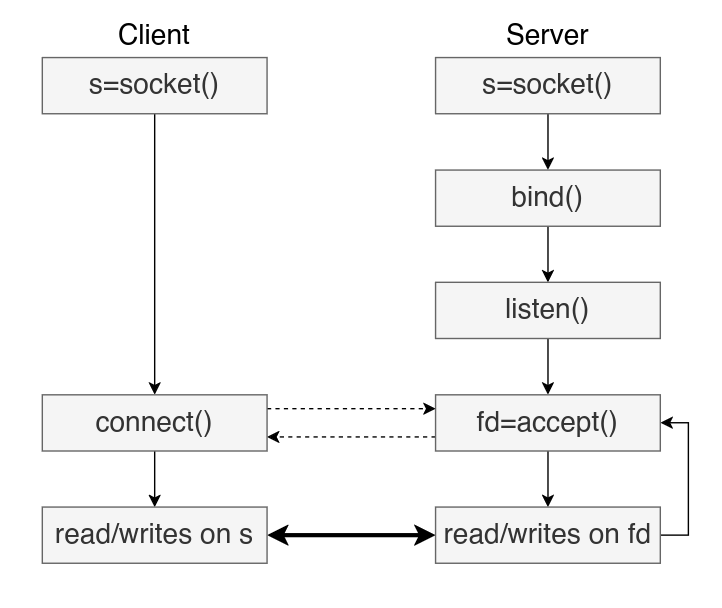
\includegraphics[width=0.5\linewidth]{Images/Socket_Programming/Socket.png}
    \caption{Connessione e comunicazione con socket.}
\end{figure}

Per le connessioni UDP, a differenza delle connessioni TCP, non c'è bisogno di mettersi in ascolto. Si possono mandare dati e ricevere dati direttamente sulla rete, usando:

\begin{cbox}
rrecvfrom(sockfd, *buf, size, flags, *src_addr, *addrlen)
sendto(sockfd, *buf, size, flags, *dst_addr, addrlen)
\end{cbox}
Queste funzioni sostituiscono le syscall write() e read().

\subsection{Codice C Server Side:}
\begin{cbox}
/* A simple server using TCP
The port number is passed as an argument */

#include <stdio.h>
#include <stdlib.h>
#include <unistd.h>
#include <string.h>
#include <sys/types.h>
#include <sys/socket.h>
#include <netinet/in.h>

void error(char *msg){
    perror(msg);
    exit(1);
}

int main(int argc, char *argv[]){
    int sockfd, newsockfd, portno, clilen;
    char buffer[256];
    struct sockaddr_in serv_addr, cli_addr;
    int n;
    
    if (argc < 2) {
        fprintf(stderr,"ERROR, no port provided\n");
        exit(1);
    }
    
    sockfd = socket(AF_INET, SOCK_STREAM, 0);
    if (sockfd < 0)
        error("ERROR opening socket");
        
    bzero((char *) &serv_addr, sizeof(serv_addr));
    portno = atoi(argv[1]);
    serv_addr.sin_family = AF_INET;
    serv_addr.sin_addr.s_addr = INADDR_ANY;
    serv_addr.sin_port = htons(portno);
    
    if (bind(sockfd, (struct sockaddr *) &serv_addr, sizeof(serv_addr)) < 0)
        error("ERROR on binding");
    
    listen(sockfd, 5);
    clilen = sizeof(cli_addr);
    newsockfd = accept(sockfd, (struct sockaddr *) &cli_addr, &clilen);
    if (newsockfd < 0) 
        error("ERROR on accept");
    
    bzero(buffer, 256);
    n = read(newsockfd, buffer, 255);
    if (n < 0)
        error("ERROR reading from socket");
        
    printf("Here is the message: %s\n",buffer);
    n = write(newsockfd, "I got your message",18);
    if (n < 0)
        error("ERROR writing to socket");
    
    return 0;
}
\end{cbox}

\subsection{Codice C Client Side:}
\begin{cbox}
#include <stdio.h>
#include <unistd.h>
#include <stdlib.h>
#include <string.h>
#include <sys/types.h>
#include <sys/socket.h>
#include <netinet/in.h>
#include <netdb.h>

void error(char *msg){
    perror(msg);
    exit(0);
}

int main(int argc, char *argv[]){
    int sockfd, portno, n;
    struct sockaddr_in serv_addr;
    struct hostent *server;
    char buffer[256];
    
    if (argc < 3) {
        fprintf(stderr,"usage %s hostname port\n", argv[0]);
        exit(0);
    }
    
    portno = atoi(argv[2]);
    sockfd = socket(AF_INET, SOCK_STREAM, 0);
    if (sockfd < 0)
        error("ERROR opening socket");

    server = gethostbyname(argv[1]);
    if (server == NULL) {
        fprintf(stderr,"ERROR, no such host\n");
        exit(0);
    }
    
    bzero((char *) &serv_addr, sizeof(serv_addr));
    serv_addr.sin_family = AF_INET;
    bcopy((char *)server->h_addr, (char *)&serv_addr.sin_addr.s_addr, server->h_length);
    serv_addr.sin_port = htons(portno);

    if (connect(sockfd, (const struct sockaddr *) &serv_addr, sizeof(serv_addr) < 0)
        error("ERROR connecting");
    
    printf("Please enter the message: ");
    bzero(buffer, 256);
    fgets(buffer, 255, stdin);
    n = write(sockfd, buffer, strlen(buffer));
    if (n < 0)
        error("ERROR writing to socket");
    
    bzero(buffer, 256);
    n = read(sockfd, buffer, 255);
    if (n < 0)
        error("ERROR reading from socket");
    printf("%s\n", buffer);
    
    return 0;
}
\end{cbox}

\subsection{Codice Python Server Side:}
\begin{pybox}
#!/usr/bin/env python3
import socket
import sys
import time

HOST = '127.0.0.1' # Standard loopback interface address (localhost)
PORT = int(sys.argv[1]) # Port to listen on

with socket.socket(socket.AF_INET, socket.SOCK_STREAM) as s:
    s.bind((HOST, PORT))
    s.listen()
    conn, addr = s.accept()
    #print('Connected by', addr)
    data = conn.recv(1024)
    print('Here is the message: %s'% data.decode('utf-8'))
    conn.sendall('I got your message'.encode('utf-8'))
    # socket must be closed by client! sleep for 1 second
    time.sleep(1) # otherwise socket goes to TIME_WAIT!
\end{pybox}

\subsection{Codice Python Client Side:}
\begin{pybox}
#!/usr/bin/env python3
import socket
import sys
HOST=sys.argv[1]
PORT=int(sys.argv[2])
with socket.socket(socket.AF_INET, socket.SOCK_STREAM) as s:
    s.connect((HOST, PORT))
    msg = input('Please enter the message: ')
    s.sendall(msg.encode('utf-8'))
    data = s.recv(1024)
    s.close()
    print('Received: %s'% data.decode('utf-8'))
\end{pybox}